\chapter{Wilsonian Effective Actions and Exact Cutoff Flow}
\label{ch:vol2-wilsonian-effective-actions}
\ConventionsEuclidean


\section{Smooth Cutoffs and Effective Actions}

We work in Euclidean signature on \(\R^D\), first for one real scalar field.
Fourier transforms are normalized by
\[
  \phi(x)=\int\frac{\dd^Dk}{(2\pi)^D}\,
  \ee^{\ii k\cdot x}\widetilde\phi(k),
  \qquad
  \widetilde\phi(k)=\int\dd^Dx\,\ee^{-\ii k\cdot x}\phi(x).
\]
For compactness, write
\[
  \int_k F(k):=\int\frac{\dd^Dk}{(2\pi)^D}\,F(k),
  \qquad
  \frac{\delta\widetilde\phi(p)}{\delta\widetilde\phi(k)}
  =(2\pi)^D\delta^{(D)}(p-k).
\]

Let \(\chi:[0,\infty)\to[0,\infty)\) be a smooth cutoff profile such that
\(\chi(t)=1+O(t)\) for \(t\ll 1\) and \(\chi(t)\) decreases rapidly for
\(t\gg 1\).  At cutoff scale \(\Lambda>0\), define
\[
  \chi_\Lambda(k):=\chi(k^2/\Lambda^2),
  \qquad
  C_\Lambda(k):=\frac{\chi_\Lambda(k)}{k^2+m^2}.
\]
Here \(m^2\geq0\) is the mass parameter in the quadratic kernel.  The
Wilsonian action at scale \(\Lambda\) is written
\begin{equation}
  S_\Lambda[\phi]
  =
  S_{\mathrm{kin},\Lambda}[\phi]+L_\Lambda[\phi],
  \label{eq:wilsonian-action-split}
\end{equation}
where
\begin{equation}
  S_{\mathrm{kin},\Lambda}[\phi]
  =
  \frac12\int_k
  \widetilde\phi(-k)\,
  \frac{k^2+m^2}{\chi_\Lambda(k)}\,
  \widetilde\phi(k).
  \label{eq:smooth-cutoff-kinetic-term}
\end{equation}
Perturbation theory around this Gaussian measure uses \(C_\Lambda(k)\) as
propagator.  The cutoff is therefore part of the definition of the covariance,
so every propagator in the Gaussian expansion carries the same regulated
kernel.

\begin{figure}[H]
  \centering
  \resizebox{0.98\textwidth}{!}{%
  \begin{tikzpicture}[x=1cm,y=1cm,every node/.style={font=\scriptsize}]
    \begin{scope}
      \node[font=\small] at (2.2,2.82) {smooth cutoff profile};
      \draw[-{Latex[length=2mm]}] (-0.15,0)--(4.4,0)
        node[below] {\(t=k^2/\Lambda^2\)};
      \draw[-{Latex[length=2mm]}] (0,-0.15)--(0,2.25)
        node[left] {\(\chi(t)\)};
      \draw[dashed,gray] (1.65,0)--(1.65,1.55);
      \draw[dashed,gray] (0,1.55)--(1.65,1.55);
      \node[below] at (1.65,-0.03) {\(1\)};
      \node[left] at (-0.03,1.55) {\(1\)};
      \draw[blue!65!black,very thick]
        (0,1.55)--(1.28,1.55)
        .. controls (1.55,1.54) and (1.62,1.15) .. (1.72,0.62)
        .. controls (1.84,0.10) and (2.45,0.04) .. (4.0,0.04);
      \node[align=center,blue!65!black] at (1.35,2.02)
        {low momenta\\unchanged};
      \node[align=center,blue!65!black] at (3.2,0.72)
        {rapid\\suppression};
    \end{scope}

    \begin{scope}[shift={(5.35,0)}]
      \node[font=\small] at (2.2,2.82) {lowering the cutoff};
      \draw[-{Latex[length=2mm]}] (-0.15,0)--(4.45,0)
        node[below] {\(|k|\)};
      \draw[-{Latex[length=2mm]}] (0,-0.15)--(0,2.25);
      \fill[orange!35,opacity=0.50]
        (1.95,0.04) rectangle (2.85,1.48);
      \draw[green!50!black,very thick]
        (0,1.55)--(1.65,1.55)
        .. controls (1.88,1.53) and (1.96,1.12) .. (2.06,0.62)
        .. controls (2.18,0.10) and (2.78,0.04) .. (4.05,0.04);
      \draw[orange!85!black,very thick]
        (0,1.55)--(2.55,1.55)
        .. controls (2.78,1.53) and (2.86,1.12) .. (2.96,0.62)
        .. controls (3.08,0.10) and (3.62,0.04) .. (4.05,0.04);
      \draw[dashed] (1.95,0)--(1.95,1.22);
      \draw[dashed] (2.85,0)--(2.85,1.22);
      \node[below] at (1.95,-0.03) {\(\Lambda'\)};
      \node[below] at (2.85,-0.03) {\(\Lambda\)};
      \node[green!50!black] at (1.0,1.25) {\(\chi_{\Lambda'}\)};
      \node[orange!85!black] at (3.45,1.12) {\(\chi_\Lambda\)};
      \node[align=center,fill=white,inner sep=2pt] at (2.45,1.86)
        {shell covariance\\\(C_\Lambda-C_{\Lambda'}\)};
    \end{scope}
  \end{tikzpicture}
  }
  \caption{A smooth cutoff profile equals one for small momentum and suppresses
  modes above \(\Lambda\).  When the cutoff is lowered to \(\Lambda'\), the
  difference of covariances is concentrated in the momentum shell between the
  two scales.}
  \label{fig:wilsonian-smooth-cutoff}
\end{figure}

The interaction functional \(L_\Lambda\) is an arbitrary translation-invariant
functional compatible with the imposed symmetries.  In a finite spatial
volume with a finite momentum cutoff, \(L_\Lambda\) is an ordinary smooth or
polynomial function of finitely many Fourier modes.  Its vertex expansion is
\begin{align}
  L_\Lambda[\phi]
  &=
  \sum_{n\geq0}\frac1{n!}
  \int\prod_{i=1}^{n-1}\frac{\dd^Dk_i}{(2\pi)^D}\,
  L_\Lambda^{(n)}(k_1,\ldots,k_{n-1})
  \notag\\
  &\hspace{3.35cm}\times
  \widetilde\phi(k_1)\cdots\widetilde\phi(k_{n-1})
  \widetilde\phi(-k_1-\cdots-k_{n-1}).
  \label{eq:general-wilsonian-interaction}
\end{align}
The coefficient functions \(L_\Lambda^{(n)}\) are symmetric in their \(n\)
external momenta after the momentum-conserving argument is restored.  Locality
of the Wilsonian action means that, for momenta small compared with
\(\Lambda\), these coefficient functions admit an expansion in polynomials of
the external momenta, with the nonpolynomial dependence controlled at the
cutoff scale.  The derivative expansion supplies an infinite set of local
coordinates organized by powers of momentum over \(\Lambda\).

The source-dependent generating functional at cutoff \(\Lambda\) is
\begin{equation}
  Z_\Lambda[J]
  =
  \int[D\phi]\,
  \exp\left[
    -S_{\mathrm{kin},\Lambda}[\phi]
    -L_\Lambda[\phi]
    -\int\dd^Dx\,J(x)\phi(x)
  \right].
  \label{eq:wilsonian-z-lambda}
\end{equation}
The Wilsonian condition for lowering \(\Lambda\) to \(\Lambda'<\Lambda\) is
the equality
\begin{equation}
  Z_{\Lambda'}[J]=Z_\Lambda[J]
  \label{eq:low-momentum-generating-function-preserved}
\end{equation}
for all sources whose Fourier transform \(\widetilde J(k)\) is supported in the
low-momentum region \(|k|<\Lambda'\), or more generally in a region where the
new cutoff profile is indistinguishable from one.  Thus the scale label on
\(S_\Lambda\) is a label on a description of the same low-momentum correlation
functions.

\section{Lowering the Cutoff}

The exact Wilsonian step is most transparent with a finite regulator.  Let
\(E_\Lambda\) be the finite-dimensional real vector space of Fourier modes
retained by the ultraviolet regulator, and let \(\dd\mu_{C_\Lambda}\) be the
centered Gaussian measure with covariance \(C_\Lambda\) on this space.  If
\[
  C_\Lambda=C_{\Lambda'}+\widehat C_{\Lambda,\Lambda'}
\]
with both summands positive covariances on the regulated vector space, then
the Gaussian convolution identity says
\begin{equation}
  \int_{E_\Lambda}F(\phi)\,\dd\mu_{C_\Lambda}(\phi)
  =
  \int_{E_{\Lambda'}}\int_{\widehat E_{\Lambda,\Lambda'}}
  F(\phi'+\phi_{\mathrm{sh}})\,
  \dd\mu_{\widehat C_{\Lambda,\Lambda'}}(\phi_{\mathrm{sh}})\,
  \dd\mu_{C_{\Lambda'}}(\phi')
  \label{eq:finite-regulator-gaussian-convolution}
\end{equation}
for every integrable regulated function \(F\).  Equation
\eqref{eq:finite-regulator-gaussian-convolution} is a theorem about Gaussian
measures on finite-dimensional vector spaces.  The continuum notation below is
the shorthand obtained by applying this identity at each regulator and then
studying the regulator-removal limit.

The algebraic step behind Wilsonian RG is the covariance identity
\begin{equation}
  C_\Lambda(k)
  =
  C_{\Lambda'}(k)+\widehat C_{\Lambda,\Lambda'}(k),
  \qquad
  \widehat C_{\Lambda,\Lambda'}(k)
  :=
  \frac{\chi_\Lambda(k)-\chi_{\Lambda'}(k)}{k^2+m^2}.
  \label{eq:wilsonian-covariance-split}
\end{equation}
The first covariance belongs to a low field \(\phi'\).  The second covariance
belongs to an independent shell field \(\phi_{\mathrm{sh}}\), with kinetic term
\begin{equation}
  \widehat S_{\mathrm{kin}}[\phi_{\mathrm{sh}}]
  =
  \frac12\int_k
  \widetilde\phi_{\mathrm{sh}}(-k)\,
  \frac{k^2+m^2}{\chi_\Lambda(k)-\chi_{\Lambda'}(k)}\,
  \widetilde\phi_{\mathrm{sh}}(k).
  \label{eq:shell-kinetic-term}
\end{equation}
The shell field is denoted \(\phi_{\mathrm{sh}}\).  A tilde denotes
Fourier transformation; thus \(\widetilde\phi_{\mathrm{sh}}(k)\) is the shell
field's Fourier mode, while \(\widetilde\phi(k)\) elsewhere is the Fourier mode
of the active field variable \(\phi\).

\begin{figure}[H]
  \centering
  \resizebox{0.98\textwidth}{!}{%
  \begin{tikzpicture}[x=1cm,y=1cm,every node/.style={font=\scriptsize}]
    \node[font=\small] at (0,2.55) {propagator identity};
    \draw[very thick] (-2.4,1.25)--(-1.2,1.25);
    \node at (-1.82,1.55) {\(C_\Lambda\)};
    \node at (-0.9,1.25) {\(=\)};
    \draw[very thick,green!50!black] (-0.55,1.25)--(0.65,1.25);
    \node[green!50!black] at (0.05,1.55) {\(C_{\Lambda'}\)};
    \node at (0.98,1.25) {\(+\)};
    \draw[very thick,orange!85!black,dashed] (1.35,1.25)--(2.55,1.25);
    \node[orange!85!black] at (1.95,1.55) {\(\widehat C_{\Lambda,\Lambda'}\)};
    \node[align=center,green!50!black] at (0.05,0.42) {low field\\\(\phi'\)};
    \node[align=center,orange!85!black] at (1.95,0.42) {shell field\\\(\phi_{\mathrm{sh}}\)};

    \begin{scope}[shift={(5.10,0)}]
      \node[font=\small] at (1.30,2.55) {shell integration};
      \draw[rounded corners=4pt,thick] (0,0.58) rectangle (2.60,1.68);
      \node at (1.30,1.13) {\(L_\Lambda[\phi'+\phi_{\mathrm{sh}}]\)};
      \draw[green!50!black,thick] (0,1.40)--(-0.72,1.82);
      \draw[green!50!black,thick] (0,0.82)--(-0.72,0.42);
      \draw[green!50!black,thick] (2.60,1.40)--(3.32,1.82);
      \draw[green!50!black,thick] (2.60,0.82)--(3.32,0.42);
      \draw[orange!85!black,thick,dashed]
        (2.05,1.60) .. controls (3.05,1.98) and (3.05,0.32) .. (2.05,0.68);
      \node[green!50!black] at (1.30,2.03) {external low modes};
      \node[orange!85!black,align=center] at (3.62,1.34)
        {contract\\shell modes};
      \draw[-{Latex[length=2mm]},thick] (4.12,1.05)--(4.85,1.05);
    \end{scope}

    \begin{scope}[shift={(10.85,0)}]
      \node[font=\small] at (0,2.55) {new interaction};
      \draw[rounded corners=4pt,thick,green!50!black] (-1.30,0.58) rectangle (1.30,1.68);
      \node[green!50!black] at (0,1.13) {\(L_{\Lambda'}[\phi']\)};
      \draw[green!50!black,thick] (-1.30,1.40)--(-2.02,1.82);
      \draw[green!50!black,thick] (-1.30,0.82)--(-2.02,0.42);
      \draw[green!50!black,thick] (1.30,1.40)--(2.02,1.82);
      \draw[green!50!black,thick] (1.30,0.82)--(2.02,0.42);
      \node[align=center,green!50!black] at (0,0.02)
        {all remaining legs\\carry low momenta};
    \end{scope}
  \end{tikzpicture}
  }
  \caption{The old Gaussian covariance can be realized as the covariance of
  two independent fields.  Integrating the shell field contracts the dashed
  propagators and produces a new interaction for the low field.}
  \label{fig:propagator-split-shell-integration}
\end{figure}

Before the support of the source is used, the covariance split rewrites the
cutoff-\(\Lambda\) functional as
\begin{align}
  Z_\Lambda[J]
  &=
  \int[D\phi']\,
  \exp\left[
    -S_{\mathrm{kin},\Lambda'}[\phi']
  \right]
  \int[D\phi_{\mathrm{sh}}]\,
  \exp\left[
    -\widehat S_{\mathrm{kin}}[\phi_{\mathrm{sh}}]
    -L_\Lambda[\phi'+\phi_{\mathrm{sh}}]
  \right]
  \notag\\
  &\hspace{2.0cm}\times
  \exp\left[
    -\int\dd^Dx\,J(x)\bigl(\phi'(x)+\phi_{\mathrm{sh}}(x)\bigr)
  \right].
  \label{eq:z-lambda-after-shell-split}
\end{align}
The condition on \(J\) is now used in its precise regulated meaning: the source
belongs to the low subspace, while the shell covariance belongs to the
complement.  Equivalently, in Fourier notation
\(\int\dd^Dx\,J(x)\phi_{\mathrm{sh}}(x)=0\) for the shell field.  With a smooth
cutoff profile one enforces this by choosing the source momenta in a slightly
smaller region on which the shell covariance vanishes, or by using a profile
with a plateau.  Thus the source term in
\eqref{eq:z-lambda-after-shell-split} couples only to \(\phi'\).  The shell
field may then be integrated out by the defining identity
\begin{equation}
  \exp\{-L_{\Lambda'}[\phi']\}
  =
  \int[D\phi_{\mathrm{sh}}]\,
  \exp\left[
    -\widehat S_{\mathrm{kin}}[\phi_{\mathrm{sh}}]
    -L_\Lambda[\phi'+\phi_{\mathrm{sh}}]
  \right],
  \label{eq:define-lambda-prime-interaction}
\end{equation}
up to a \(\phi'\)-independent normalization.  Combining
\eqref{eq:shell-kinetic-term} and
\eqref{eq:define-lambda-prime-interaction} with the Gaussian measure for
\(\phi'\) gives \eqref{eq:low-momentum-generating-function-preserved}.  The
definition is exact for each finite regulator by
\eqref{eq:finite-regulator-gaussian-convolution}.  Perturbation theory expands
the logarithm of the shell expectation in connected shell contractions, and
the continuum claim is the existence of the corresponding limit after the
renormalization conditions have been imposed.

\section{The Wilson-Polchinski Equation}

Let \(\Lambda'\) approach \(\Lambda\).  The shell covariance becomes
infinitesimal, and the definition of \(L_{\Lambda'}\) becomes a differential
equation.  With \(C_\Lambda(k)=\chi_\Lambda(k)/(k^2+m^2)\) and with the
functional-derivative convention already stated, the interaction functional
satisfies
\begin{equation}
  \Lambda\partial_\Lambda L_\Lambda[\phi]
  =
  \frac12\int_k
  \Lambda\partial_\Lambda C_\Lambda(k)
  \left[
    \frac{\delta L_\Lambda}{\delta\widetilde\phi(k)}
    \frac{\delta L_\Lambda}{\delta\widetilde\phi(-k)}
    -
    \frac{\delta^2 L_\Lambda}
      {\delta\widetilde\phi(k)\delta\widetilde\phi(-k)}
  \right].
  \label{eq:wilson-polchinski-flow}
\end{equation}
In \eqref{eq:wilson-polchinski-flow}, \(\widetilde\phi(k)\) denotes the Fourier
mode of the remaining field.  The notation matches the functional derivative
convention; after the infinitesimal shell has been integrated, there is again
only one field argument of \(L_\Lambda\).

Since
\[
  \Lambda\partial_\Lambda C_\Lambda(k)
  =
  \frac{\Lambda\partial_\Lambda\chi(k^2/\Lambda^2)}{k^2+m^2},
\]
the integration kernel is supported where the cutoff profile changes, namely
near \(|k|\simeq\Lambda\) for a rapidly decreasing smooth cutoff.  The two
terms in \eqref{eq:wilson-polchinski-flow} have a direct graphical meaning:
the product of first derivatives joins two vertices by one shell propagator,
whereas the second derivative contracts two legs of a single vertex.

\begin{figure}[H]
  \centering
  \resizebox{0.95\textwidth}{!}{%
  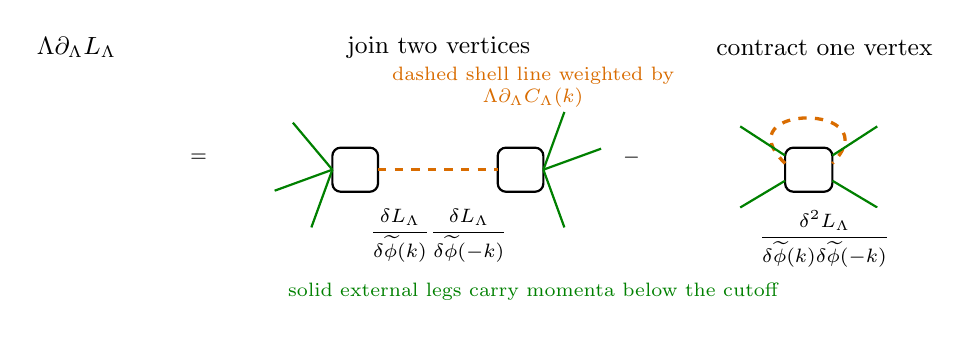
\begin{tikzpicture}[x=1cm,y=1cm,every node/.style={font=\scriptsize}]
    \node[font=\small] at (0,2.55)
      {\(\Lambda\partial_\Lambda L_\Lambda\)};
    \node at (1.55,1.15) {\(=\)};

    \begin{scope}[shift={(3.25,0)}]
      \node[font=\small] at (1.35,2.55) {join two vertices};
      \draw[rounded corners=3pt,thick] (0.0,0.72) rectangle (0.58,1.28);
      \draw[rounded corners=3pt,thick] (2.10,0.72) rectangle (2.68,1.28);
      \draw[orange!85!black,very thick,dashed] (0.58,1.0)--(2.10,1.0);
      \foreach \a in {130,200,250} {
        \draw[green!50!black,thick] (0.0,1.0)--+(\a:0.78);
      }
      \foreach \a in {-70,20,70} {
        \draw[green!50!black,thick] (2.68,1.0)--+(\a:0.78);
      }
      \node[align=center] at (1.35,0.16)
        {\(\displaystyle
        \frac{\delta L_\Lambda}{\delta\widetilde\phi(k)}
        \frac{\delta L_\Lambda}{\delta\widetilde\phi(-k)}\)};
    \end{scope}

    \node at (7.05,1.15) {\(-\)};

    \begin{scope}[shift={(8.25,0)}]
      \node[font=\small] at (1.25,2.55) {contract one vertex};
      \draw[rounded corners=3pt,thick] (0.75,0.72) rectangle (1.35,1.28);
      \draw[orange!85!black,very thick,dashed]
        (0.75,1.08) .. controls (-0.05,1.85) and (2.10,1.85) .. (1.35,1.08);
      \draw[green!50!black,thick] (0.75,1.18)--(0.18,1.55);
      \draw[green!50!black,thick] (0.75,0.86)--(0.18,0.52);
      \draw[green!50!black,thick] (1.35,1.18)--(1.92,1.55);
      \draw[green!50!black,thick] (1.35,0.86)--(1.92,0.52);
      \node[align=center,fill=white,inner sep=1pt] at (1.25,0.12)
        {\(\displaystyle
        \frac{\delta^2 L_\Lambda}
        {\delta\widetilde\phi(k)\delta\widetilde\phi(-k)}\)};
    \end{scope}

    \node[orange!85!black,align=center,fill=white,inner sep=1pt] at (5.8,2.05)
      {dashed shell line weighted by\\\(\Lambda\partial_\Lambda C_\Lambda(k)\)};
    \node[green!50!black] at (5.8,-0.55) {solid external legs carry momenta below the cutoff};
  \end{tikzpicture}
  }
  \caption{The exact cutoff flow has two local operations.  The first term
  connects two interaction vertices with an infinitesimal shell propagator.
  The second term contracts two legs belonging to the same interaction
  vertex.}
  \label{fig:wilson-polchinski-diagrams}
\end{figure}

Equation \eqref{eq:wilson-polchinski-flow} is a closed equation on the
functional \(L_\Lambda\).  In a local coordinate system on theory space it is
an infinite coupled system of differential equations for the coefficients of
all local operators.  The use of a smooth cutoff is important: it keeps the
infinitesimal shell operation compatible with a derivative expansion at
external momenta small compared with \(\Lambda\).

The sign in \eqref{eq:wilson-polchinski-flow} is fixed by the direction of the
cutoff derivative.  For \(\Lambda'=\Lambda-\delta\Lambda\), the shell covariance
is
\[
  \delta C(k)
  =
  C_\Lambda(k)-C_{\Lambda'}(k)
  =
  \delta\Lambda\,\partial_\Lambda C_\Lambda(k)+O(\delta\Lambda^2).
\]
The Gaussian convolution formula gives, to first order in \(\delta\Lambda\),
\[
  \ee^{-L_{\Lambda-\delta\Lambda}[\phi]}
  =
  \left[
    1+
    \frac12\int_k
    \delta\Lambda\,\partial_\Lambda C_\Lambda(k)
    \frac{\delta^2}
      {\delta\widetilde\phi(k)\delta\widetilde\phi(-k)}
  \right]
  \ee^{-L_\Lambda[\phi]} .
\]
Since
\[
  \frac{\delta^2\ee^{-L_\Lambda}}
    {\delta\widetilde\phi(k)\delta\widetilde\phi(-k)}
  =
  \left[
    \frac{\delta L_\Lambda}{\delta\widetilde\phi(k)}
    \frac{\delta L_\Lambda}{\delta\widetilde\phi(-k)}
    -
    \frac{\delta^2L_\Lambda}
      {\delta\widetilde\phi(k)\delta\widetilde\phi(-k)}
  \right]\ee^{-L_\Lambda},
\]
and
\[
  L_{\Lambda-\delta\Lambda}
  =
  L_\Lambda-\delta\Lambda\,\partial_\Lambda L_\Lambda+O(\delta\Lambda^2),
\]
the displayed Wilson-Polchinski equation follows.  This derivation is an
identity for the regulated finite-dimensional Gaussian integral; the continuum
notation suppresses the regulator that makes the functional derivatives
ordinary derivatives on a finite vector space.

\section{Linearized Flow and Scaling Coordinates}

A fixed point of the Wilsonian flow is a scale-invariant interaction
\(L_*\) after all quantities have been written in dimensionless coordinates.
Let \(t=\log\Lambda\).  Near a fixed point write
\[
  L_\Lambda=L_*+\sum_I g_I(\Lambda)\,\mathcal O_I ,
\]
where \(\mathcal O_I\) are local coordinates on theory space.  The linearized
flow has the form
\[
  \frac{\dd g_I}{\dd t}
  =
  \sum_J M_I{}^J g_J+O(g^2).
\]
Choosing eigenvectors of \(M\) gives scaling coordinates \(u_\alpha\):
\begin{equation}
  \frac{\dd u_\alpha}{\dd t}
  =
  -y_\alpha u_\alpha+O(u^2).
  \label{eq:wilsonian-linearized-eigenflow}
\end{equation}
The number \(y_\alpha\) is the relevance exponent.  In the convention
\(t=\log\Lambda\), decreasing the cutoff moves toward the infrared, so
\eqref{eq:wilsonian-linearized-eigenflow} implies
\[
  u_\alpha(\Lambda)
  =
  u_\alpha(\Lambda_0)
  \left(\frac{\Lambda}{\Lambda_0}\right)^{-y_\alpha}
  +O(u^2).
\]
A coordinate with \(y_\alpha>0\) grows when \(\Lambda\) is lowered.  It is a
relevant coordinate and must be tuned to reach the critical surface, or fixed
by a renormalization condition when a continuum limit is constructed.  A
coordinate with \(y_\alpha<0\) is irrelevant: its value at a fixed physical
scale is attracted to a function of the relevant and marginal coordinates
along a renormalized trajectory.

The critical surface associated with a fixed point is the set of points whose
infrared flow approaches that fixed point.  Its codimension equals the number
of relevant directions, after quotienting redundant field redefinitions and
symmetry directions.  This is the Wilsonian meaning of tuning.  A statistical
system at a continuous transition is obtained by tuning the relevant
coordinates to the critical surface; a continuum QFT near the fixed point is
obtained by holding the relevant physical coordinates fixed while the
ultraviolet cutoff is removed.

The scaling dimension of the local operator conjugate to \(u_\alpha\) is
\[
  \Delta_\alpha=D-y_\alpha
\]
when the fixed point is conformal and the coupling multiplies
\(\int\dd^Dx\,\mathcal O_\alpha(x)\).  Thus the Wilsonian eigenvalue problem
and the conformal scaling-operator problem are the same local question seen
from two sides: flow in theory space and dilation on local operators.

\section{Redundant Directions and Field Coordinates}

Theory space is coordinatized by actions, but different coordinates can
describe the same correlation functions.  A local change of field variable
\[
  \phi(x)\longmapsto \phi(x)+\epsilon F[\phi](x)
\]
changes the action, to first order in \(\epsilon\), by
\[
  S[\phi]\longmapsto
  S[\phi]
  +
  \epsilon\int\dd^Dx\,
  \frac{\delta S}{\delta\phi(x)}F[\phi](x)
  -
  \epsilon\,\operatorname{Tr}\frac{\delta F}{\delta\phi}
  +O(\epsilon^2).
\]
The trace term is the local Jacobian contribution in a regulated functional
integral.  Operators of the form
\[
  \int\dd^Dx\,
  \frac{\delta S}{\delta\phi(x)}F[\phi](x)
  \quad
  \text{together with the associated Jacobian}
\]
generate redundant directions.  They change the coordinate representative of
the Wilsonian action and the representatives of local composite operators, but
they leave separated-point correlation functions invariant after the
corresponding field redefinition is applied.

The quotient by redundant directions is important in the linearized RG
problem.  An eigenvector of the flow that is tangent to a field redefinition
is a change of local coordinates on theory space.  Relevant, marginal, and
irrelevant directions that classify continuum limits are therefore physical
directions modulo these redundant tangent vectors, with symmetries and
operator normalizations fixed as part of the coordinate choice.

\section{Renormalized Trajectories and Universality}

Let \(u_r\) denote the relevant coordinates and \(u_i\) the irrelevant
coordinates near a fixed point.  A renormalized trajectory is a submanifold of
theory space on which the irrelevant coordinates are functions of the relevant
ones:
\[
  u_i=F_i(u_r).
\]
The functions \(F_i\) are determined by the requirement that the trajectory can
be extended toward the ultraviolet while remaining in the basin where the
fixed-point expansion is valid.  Perturbatively, they are found by solving the
irrelevant beta-function equations order by order in the relevant and marginal
coordinates.

Universality is the statement that many different microscopic actions flow to
the same renormalized trajectory at a fixed physical scale.  Suppose two bare
actions at cutoff \(\Lambda_0\) have the same relevant coordinates after
tuning, but differ by an irrelevant coordinate \(u_i(\Lambda_0)\).  Linearized
flow gives
\[
  u_i(\Lambda_R)
  =
  \left(\frac{\Lambda_R}{\Lambda_0}\right)^{-y_i}
  u_i(\Lambda_0)
  +\text{nonlinear terms},
  \qquad
  y_i<0,
\]
for a fixed reference scale \(\Lambda_R\ll\Lambda_0\).  Thus the difference in
low-energy correlation functions is suppressed by powers of
\(\Lambda_R/\Lambda_0\), after the relevant coordinates and field
normalizations have been matched.  The suppression exponent is
\(-y_i=\Delta_i-D>0\) for the first omitted irrelevant operator.

This gives a precise meaning to effective field theory.  A finite list of
relevant and marginal coordinates must be measured or tuned.  Irrelevant
operators are still present, and their coefficients encode real short-distance
physics, but their effect on low-energy observables is organized by powers of
the ratio of scales and by the symmetries that determine which operators may
appear.

\section{A Quartic-Sextic Toy Flow}

Consider the massless scalar theory in \(D=4\) and keep only two local
coordinates in the interaction,
\begin{equation}
  L_\Lambda[\phi]
  =
  \int\dd^4x\,
  \bigl(g_4(\Lambda)\phi(x)^4+g_6(\Lambda)\phi(x)^6\bigr).
  \label{eq:quartic-sextic-truncation}
\end{equation}
This is a two-dimensional projection of the full Wilsonian flow.  Numerical
normalizations of \(g_4\) and \(g_6\) are absorbed into the constants below.
The corresponding dimensionless coordinates are
\begin{equation}
  \lambda_4(\Lambda):=g_4(\Lambda),
  \qquad
  \lambda_6(\Lambda):=\Lambda^2g_6(\Lambda).
  \label{eq:lambda-four-six-definitions}
\end{equation}
The canonical term in the second equation is \(2\lambda_6\), because
\(\phi^6\) has coefficient of mass dimension \(-2\) in four dimensions.  A
projected Wilsonian beta function is, by definition,
\[
  \beta_A(\lambda):=\Lambda\frac{\dd\lambda_A}{\dd\Lambda}.
\]
The variables \(\lambda_A\) are coordinates on a chosen cutoff scheme, not
observables by themselves.  To isolate the structural point, choose local
coordinates in which the small-coupling flow begins as
\begin{equation}
  \Lambda\frac{\dd\lambda_4}{\dd\Lambda}
  =
  -a\lambda_6+\cdots,
  \qquad
  \Lambda\frac{\dd\lambda_6}{\dd\Lambda}
  =
  2\lambda_6+b\lambda_4^2+\cdots ,
  \label{eq:quartic-sextic-beta-functions}
\end{equation}
where \(a\) and \(b\) depend on the cutoff profile and on the normalization of
the two operators.  The ellipses denote terms of higher order in the retained
local coordinates and terms involving the omitted coordinates.  The coefficient
\(2\) is the canonical irrelevant eigenvalue in the convention
\(t=\log\Lambda\): at fixed dimensionful \(g_6\), the dimensionless
\(\lambda_6=\Lambda^2g_6\) decreases when the cutoff is lowered.

Assume \(\lambda_6=O(\lambda_4^2)\) along the trajectory and work to the first
nontrivial order.  Let
\[
  h(\Lambda):=\lambda_6(\Lambda)+\frac b2\lambda_4(\Lambda)^2 .
\]
Using \eqref{eq:quartic-sextic-beta-functions},
\begin{equation}
  \Lambda\frac{\dd}{\dd\Lambda}
  \left(\lambda_6+\frac b2\lambda_4^2\right)
  =
  2\left(\lambda_6+\frac b2\lambda_4^2\right)
  +O(\lambda_4h)+O(\lambda_4^3).
  \label{eq:slaving-combination}
\end{equation}
Thus, over a perturbative range in which the variation of \(\lambda_4\) only
affects this equation at higher order,
\[
  h(\Lambda)
  =
  h(\Lambda_*)\left(\frac{\Lambda}{\Lambda_*}\right)^2
  +O(\lambda_4^3).
\]
Along the flow toward the infrared, \(\Lambda\downarrow0\), the transverse
combination \(h\) is suppressed by the canonical irrelevant power.  The
attracting curve is therefore
\begin{equation}
  \lambda_6(\Lambda)
  =
  -\frac b2\lambda_4(\Lambda)^2+O(\lambda_4^3)
  \label{eq:lambda-six-slaved}
\end{equation}
on the attracting curve.  Substitution into the \(\lambda_4\) equation gives
\begin{equation}
  \Lambda\frac{\dd\lambda_4}{\dd\Lambda}
  =
  \frac{ab}{2}\lambda_4^2+O(\lambda_4^3).
  \label{eq:lambda-four-induced-beta}
\end{equation}
This equation is the induced beta function for the retained marginal
coordinate in the reduced coordinate system.  Comparison with a 1PI
renormalization convention requires an explicitly chosen finite
reparametrization between Wilsonian coordinates and the renormalized coupling
used to label Green functions; the structural fact is that the irrelevant
coordinate has been eliminated by solving its own flow equation.

\begin{figure}[H]
  \centering
  \resizebox{0.84\textwidth}{!}{%
  \begin{tikzpicture}[x=1cm,y=1cm,every node/.style={font=\scriptsize}]
    \draw[-{Latex[length=2mm]},thick] (-0.15,0)--(6.5,0)
      node[below] {\(\lambda_4\)};
    \draw[-{Latex[length=2mm]},thick] (0,-2.15)--(0,2.35)
      node[left] {\(\lambda_6\)};
    \node[below left] at (0,0) {\((0,0)\)};

    \draw[blue!65!black,very thick,domain=0.05:5.8,samples=100]
      plot (\x,{-0.055*\x*\x});

    \foreach \y/\bend in {1.85/22,1.25/17,0.70/12,-0.55/-10,-1.35/-18} {
      \draw[green!45!black,thick,-{Latex[length=2mm]}]
        (5.9,\y) .. controls (4.3,{\y-0.9}) and (2.7,{-0.055*2.7*2.7+0.35*\y})
        .. (1.45,{-0.055*1.45*1.45});
    }
    \foreach \x in {1.0,1.8,2.6,3.4,4.2,5.0} {
      \draw[blue!65!black,thick,-{Latex[length=1.8mm]}]
        (\x,{-0.055*\x*\x})
        .. controls ({\x-0.30},{-0.055*\x*\x+0.04}) and ({\x-0.60},{-0.055*(\x-0.6)*(\x-0.6)})
        .. ({\x-0.82},{-0.055*(\x-0.82)*(\x-0.82)});
    }
    \node[green!45!black,align=center] at (4.95,1.85)
      {decreasing \(\Lambda\)\\flows toward the curve};
    \node[blue!65!black,align=center,fill=white,inner sep=3pt] at (4.55,-1.82)
      {\(\lambda_6=-\frac b2\lambda_4^2+O(\lambda_4^3)\)\\attracting curve};
    \node[blue!65!black] at (1.0,0.45) {IR};
  \end{tikzpicture}
  }
  \caption{In the two-coordinate projection, the irrelevant coordinate
  \(\lambda_6\) rapidly approaches a curve determined by \(\lambda_4\).  The
  arrows indicate the direction of decreasing cutoff.  The curve is drawn in
  a normalization with \(b>0\); changing the sign convention for the
  \(\phi^6\) coordinate reflects the vertical axis but not the attraction
  statement.}
  \label{fig:quartic-sextic-ir-flow}
\end{figure}

This example is deliberately modest.  It shows one structural feature of the
full equation: irrelevant local coordinates are generally generated even if
they are absent in the bare action, and near a controlled trajectory they are
determined, order by order, by the coordinates that remain to be fixed at a
reference scale.

\section{Renormalizability as a Continuum Limit}

The Wilsonian flow is a downward flow in cutoff.  If an action
\(S_{\Lambda_0}\) is given at a finite ultraviolet cutoff \(\Lambda_0\), then
\eqref{eq:define-lambda-prime-interaction} or
\eqref{eq:wilson-polchinski-flow} constructs \(S_\Lambda\) for
\(\Lambda<\Lambda_0\).  The finite-cutoff construction therefore supplies a
trajectory below \(\Lambda_0\); a description extending to arbitrarily large
\(\Lambda\) is a continuum-limit datum.

Take a regulated path integral at cutoff \(\Lambda_0\), with interaction
\begin{equation}
  L_{\Lambda_0}[\phi]
  =
  \sum_I g_I^{\mathrm{bare}}(\Lambda_0)\,O_I[\phi],
  \label{eq:bare-action-at-lambda-zero}
\end{equation}
where \(O_I\) are local operators compatible with the symmetries.  After
flowing down to a fixed reference scale \(\Lambda_R\), low-momentum Green
functions can be expressed in terms of the Wilsonian coordinates
\(g_I(\Lambda_R)\).  A continuum limit is a limit
\(\Lambda_0\to\infty\) in which the bare coordinates are chosen as functions
of \(\Lambda_0\) so that selected physical coordinates at \(\Lambda_R\) are
held fixed and the remaining Wilsonian coordinates at \(\Lambda_R\) approach
limits.

In the quartic-sextic projection, impose the ultraviolet boundary condition
\[
  \lambda_4(\Lambda_0)=\lambda_4^{\mathrm{bare}}(\Lambda_0),
  \qquad
  \lambda_6(\Lambda_0)=0,
\]
and choose \(\lambda_4^{\mathrm{bare}}(\Lambda_0)\) so that
\[
  \lambda_4(\Lambda_R)=\lambda_4^R
\]
is fixed at the reference scale.  The Wilsonian renormalizability question in
this projection is whether
\begin{equation}
  \lim_{\Lambda_0\to\infty}
  \lambda_6(\Lambda_R)
  \bigm|_{\lambda_4(\Lambda_R)=\lambda_4^R}
  \label{eq:lambda-six-continuum-limit-question}
\end{equation}
exists.  Under perturbative control, with small couplings along the trajectory
and sufficiently mild dependence of the beta functions on the irrelevant
coordinate, the limit can be seen directly from the transverse coordinate
\(h\).  The boundary condition \(\lambda_6(\Lambda_0)=0\) gives
\[
  h(\Lambda_0)
  =
  \frac b2\lambda_4(\Lambda_0)^2 .
\]
After tuning \(\lambda_4(\Lambda_R)=\lambda_4^R\), the homogeneous memory of
this ultraviolet boundary condition is
\[
  h(\Lambda_R)
  =
  h(\Lambda_0)
  \left(\frac{\Lambda_R}{\Lambda_0}\right)^2
  +O\bigl((\lambda_4^R)^3\bigr)
\]
within the perturbative domain.  Therefore
\[
  \lambda_6(\Lambda_R)
  =
  -\frac b2(\lambda_4^R)^2
  +O\bigl((\lambda_4^R)^3\bigr)
  +O\left(\left(\frac{\Lambda_R}{\Lambda_0}\right)^2\right),
\]
where the coefficient of the last term is bounded by the assumed control of
the bare trajectory.  This displays the continuum-limit mechanism: the
irrelevant coordinate at the fixed physical scale is selected by the
renormalized trajectory, while the memory of the microscopic boundary
condition is power-suppressed.

\begin{figure}[H]
  \centering
  \resizebox{0.88\textwidth}{!}{%
  \begin{tikzpicture}[x=1cm,y=1cm,every node/.style={font=\scriptsize}]
    \tikzset{
      midflow/.style={
        postaction={
          decorate,
          decoration={
            markings,
            mark=at position 0.60 with {\arrow{Latex[length=2mm]}}
          }
        }
      }
    }
    \draw[-{Latex[length=2mm]},thick] (-0.2,0)--(8.0,0)
      node[below] {\(\lambda_4\)};
    \draw[-{Latex[length=2mm]},thick] (0,-1.65)--(0,3.05)
      node[left] {\(\lambda_6\)};

    \draw[dashed,green!45!black] (1.35,-1.45)--(1.35,2.65);
    \node[green!45!black,below] at (1.35,-1.45) {\(\lambda_4^R\)};

    \draw[blue!65!black,very thick,domain=0.35:7.35,samples=120]
      plot (\x,{0.32+0.07*(\x-1.35)+0.045*(\x-1.35)*(\x-1.35)});
    \node[blue!65!black,align=center,fill=white,inner sep=2pt] at (5.6,2.38)
      {renormalized\\trajectory curve};

    \foreach \x/\y in {7.2/0,6.4/0,5.6/0,4.8/0,4.0/0} {
      \fill[purple!80!black] (\x,\y) circle (1.8pt);
      \draw[purple!80!black,thick,midflow]
        (\x,\y)
        .. controls ({0.72*\x+0.62},{1.40}) and (2.45,0.55)
        .. (1.35,0.32);
    }
    \node[purple!80!black,align=center,fill=white,inner sep=1pt] at (4.25,1.14)
      {RG flow\\toward \(\Lambda_R\)};
    \node[purple!80!black,align=center] at (5.85,-0.62)
      {bare actions\\\(\lambda_6(\Lambda_0)=0\)};

    \fill[green!45!black] (1.35,0.32) circle (2.5pt);
    \node[green!45!black,align=left,fill=white,inner sep=1pt] at (2.05,-0.32)
      {\((\lambda_4^R,\lambda_6(\Lambda_R))\)};

    \draw[-{Latex[length=2mm]},red!70!black,thick,dashed]
      (0.22,0.32)--(1.25,0.32);
    \node[red!70!black,align=center,fill=white,inner sep=2pt] at (0.72,0.85)
      {limiting value\\as \(\Lambda_0\to\infty\)};

    \node[gray!70!black] at (6.95,0.38) {\(\Lambda_0\)};
    \node[gray!70!black] at (7.35,0.82) {\(\Lambda_0'\)};
    \draw[-{Latex[length=1.7mm]},gray!70!black] (6.85,0.45)--(7.25,0.72);
    \node[gray!70!black] at (7.55,1.08) {increasing cutoff};
  \end{tikzpicture}
  }
  \caption{For each ultraviolet cutoff \(\Lambda_0\), the bare quartic
  coupling is tuned so that \(\lambda_4(\Lambda_R)=\lambda_4^R\).  The
  continuum-limit statement asks whether the induced value of
  \(\lambda_6(\Lambda_R)\) approaches a limit as \(\Lambda_0\) is removed.}
  \label{fig:continuum-limit-wilsonian}
\end{figure}

The same analysis allows a finite nonzero value of the dimensionless
irrelevant coordinate at the ultraviolet cutoff.  In the example,
\[
  g_6^{\mathrm{bare}}(\Lambda_0)
  =
  \Lambda_0^{-2}\lambda_6(\Lambda_0).
\]
Thus a finite \(\lambda_6(\Lambda_0)\) corresponds to a dimensionful bare
coefficient suppressed by the cutoff.  This is the form produced by
lattice regularizations with lattice spacing \(a=\Lambda_0^{-1}\): many local
operators are present at the cutoff scale, but after tuning the relevant and
marginal coordinates, irrelevant coordinates approach their continuum
trajectory values at fixed physical scale.
For a hypercubic lattice, the edge of the Brillouin zone is
\(\Lambda_{\rm BZ}=\pi/a=\pi\Lambda_0\).  The estimates in this chapter use
\(\Lambda_0=a^{-1}\) as the inverse-spacing cutoff convention; using
\(\Lambda_{\rm BZ}\) instead only rescales the constants multiplying
cutoff-suppressed powers.

The perturbative Wilsonian statement has explicit hypotheses.  Along the
trajectory under consideration, the couplings must remain small enough for the
local-coordinate expansion and the omitted-operator estimates to be valid; the
derivatives such as \(\partial\beta_6/\partial\lambda_6\) and
\(\partial\beta_4/\partial\lambda_4\) must remain controlled; and the beta
function for the retained marginal coordinate must vary slowly enough along
the trajectory that the irrelevant directions are genuinely suppressed.  In
this regime, the Wilsonian flow gives the structural reason that the
power-counting classification of local operators organizes perturbative
renormalization.

This finite-coordinate estimate should not be mistaken for a constructive
existence theorem for a non-Gaussian four-dimensional scalar continuum limit.
Theorem~\ref{thm:standard-four-dimensional-scalar-triviality} states that,
for the positive lattice \(\lambda\phi^4_4\) and nearest-neighbor
ferromagnetic Ising-type scaling-limit problems covered by the known
triviality theorems, the critical or near-critical continuum limits are
Gaussian.  The Wilsonian estimate above is a local perturbative
mechanism: it explains how irrelevant coordinates lose memory of their
finite-cutoff boundary values when a controlled trajectory with fixed
renormalized coordinates is assumed.  It does not prove that such a controlled
trajectory exists to arbitrarily high cutoff at nonzero renormalized quartic
coupling.  The constructive theorem says that, for the specified standard
families and covered critical regimes, the limiting connected correlations
beyond the two-point function vanish.

\section{A Local Estimate for Cutoff Removal}

The quartic-sextic example is the one-dimensional irrelevant-coordinate
version of a general local estimate.  This estimate is a finite-coordinate
statement: choose a projection of the Wilsonian action onto local coordinates
\[
  z=(u,v)\in U\times V,
\]
where \(u=(u^1,\ldots,u^r)\) are the coordinates fixed by renormalization
conditions at the reference scale \(\Lambda_R\), and
\(v=(v^1,\ldots,v^s)\) are irrelevant coordinates retained in the projection.
Let
\[
  t=\log\Lambda,\qquad
  t_R=\log\Lambda_R,\qquad
  t_0=\log\Lambda_0 .
\]
In the coordinate neighborhood under consideration, write the projected flow
as
\begin{equation}
  \frac{\dd u^a}{\dd t}=B^a(u,v),
  \qquad
  \frac{\dd v^\rho}{\dd t}
  =
  A^\rho{}_\sigma v^\sigma+F^\rho(u,v).
  \label{eq:finite-coordinate-wilsonian-flow-split}
\end{equation}
The matrix \(A\) is the linear irrelevant block.  In the convention
\(t=\log\Lambda\), an irrelevant coordinate has a positive eigenvalue in
\(A\); the flow is therefore contracting in that coordinate when the cutoff
is lowered from \(t_0\) to \(t_R<t_0\).  We assume a norm on \(V\) and
constants \(C_A,\omega>0\) such that
\begin{equation}
  \|e^{A\tau}\|
  \leq
  C_A e^{\omega\tau},
  \qquad
  \tau\leq0 .
  \label{eq:irrelevant-backward-semigroup-bound}
\end{equation}
Thus \(e^{A(t_R-t_0)}\) is bounded by
\[
  C_A\left(\frac{\Lambda_R}{\Lambda_0}\right)^\omega .
\]

For a solution of \eqref{eq:finite-coordinate-wilsonian-flow-split} on
\([t_R,t_0]\), variation of constants gives
\begin{equation}
  v(t_R)
  =
  e^{A(t_R-t_0)}v(t_0)
  -
  \int_{t_R}^{t_0}
  e^{A(t_R-s)}F(u(s),v(s))\,\dd s .
  \label{eq:irrelevant-coordinate-variation-of-constants}
\end{equation}
The first term is the direct memory of the irrelevant bare coordinate.  The
second term is generated by the flow along the trajectory.  These two terms
have different logical roles: suppression of the first term follows from the
irrelevant eigenvalues, while existence of the cutoff-removal limit requires
control of the generated integral and of the tuning used to hold \(u(t_R)\)
fixed.

\begin{proposition}[Suppression of irrelevant boundary memory]
Assume \eqref{eq:irrelevant-backward-semigroup-bound}.  If the irrelevant bare
coordinate satisfies \(\|v(t_0)\|\leq M\) uniformly in \(t_0\), then the direct
boundary contribution to \(v(t_R)\) obeys
\[
  \|e^{A(t_R-t_0)}v(t_0)\|
  \leq
  C_A M
  \left(\frac{\Lambda_R}{\Lambda_0}\right)^\omega .
\]
If the first omitted irrelevant coordinate has exponent \(\omega_{\rm min}\),
then the same estimate begins with the power
\((\Lambda_R/\Lambda_0)^{\omega_{\rm min}}\).
\end{proposition}

\begin{proof}
Set \(\tau=t_R-t_0\leq0\) in
\eqref{eq:irrelevant-backward-semigroup-bound}.  Since
\(\exp[\omega(t_R-t_0)]=(\Lambda_R/\Lambda_0)^\omega\), the displayed
estimate follows immediately.
\end{proof}

The generated term in
\eqref{eq:irrelevant-coordinate-variation-of-constants} is the part that
selects the continuum graph.  The precise finite-coordinate hypothesis is the
existence, after tuning the retained bare coordinates, of a limit
\begin{equation}
  V^\rho_R(u_R)
  =
  \lim_{\Lambda_0\to\infty}
  \left[
    -
    \int_{t_R}^{t_0}
    \left(e^{A(t_R-s)}F(u(s),v(s))\right)^\rho
    \dd s
  \right],
  \label{eq:continuum-graph-generated-irrelevant-coordinate}
\end{equation}
where the trajectory is constrained by
\[
  u(t_R)=u_R .
\]
When this limit exists uniformly for \(u_R\) in a small coordinate
neighborhood, the finite projection of the renormalized trajectory at
\(\Lambda_R\) is the graph
\[
  v^\rho=V^\rho_R(u_R).
\]
For finite \(\Lambda_0\), define the generated-integral remainder
\[
  R_F(t_0;u_R)
  =
  -
  \int_{t_R}^{t_0}
  e^{A(t_R-s)}F(u(s),v(s))\,\dd s
  -
  V_R(u_R).
\]

\begin{proposition}[Finite-coordinate cutoff-removal estimate]
Fix \(u_R\) and suppose that, for every sufficiently large \(t_0\), the
retained bare coordinates can be tuned so that \(u(t_R)=u_R\).  Assume:
\begin{enumerate}[label=(\roman*)]
  \item the solution remains in a coordinate neighborhood where
  \eqref{eq:finite-coordinate-wilsonian-flow-split} is valid;
  \item the irrelevant semigroup satisfies
  \eqref{eq:irrelevant-backward-semigroup-bound};
  \item the irrelevant bare coordinates are uniformly bounded;
  \item the generated integral in
  \eqref{eq:continuum-graph-generated-irrelevant-coordinate} converges
  uniformly with
  \[
    \|R_F(t_0;u_R)\|
    \leq
    C_F\left(\frac{\Lambda_R}{\Lambda_0}\right)^{\omega_F}
  \]
  for some \(C_F,\omega_F>0\).
\end{enumerate}
Then the irrelevant coordinates at the reference scale have the form
\[
  v(t_R)
  =
  V_R(u_R)
  +
  O\!\left[
    \left(\frac{\Lambda_R}{\Lambda_0}\right)^{\min(\omega,\omega_F)}
  \right],
  \qquad
  \Lambda_0\to\infty ,
\]
with the exponent replaced by the smallest retained irrelevant exponent when
several irrelevant coordinates are present.
\end{proposition}

\begin{proof}
Equation \eqref{eq:irrelevant-coordinate-variation-of-constants} writes
\(v(t_R)\) as the sum of the boundary contribution and the generated
contribution.  The preceding proposition bounds the boundary contribution by
\((\Lambda_R/\Lambda_0)^\omega\).  The generated contribution is
\(V_R(u_R)+R_F(t_0;u_R)\), with \(R_F\) bounded by the fourth hypothesis.
Combining the two estimates gives the stated asymptotic form.
\end{proof}

The hypotheses of the proposition are the mathematical content of a
Wilsonian continuum-limit argument in a chosen local projection.  The tuning
condition \(u(t_R)=u_R\) is a statement about the endpoint map from bare
coordinates at \(\Lambda_0\) to renormalized coordinates at \(\Lambda_R\).
In perturbation theory this endpoint map is usually solved order by order.
When the linearized endpoint map in the retained coordinates is invertible,
the implicit function theorem gives the local tuning functions at finite
\(\Lambda_0\).  The remaining task is to prove estimates, uniform in
\(\Lambda_0\), that keep the trajectory in the assumed coordinate
neighborhood and make the generated integral converge.

\begin{remark}[Renormalons and Wilsonian data]
Assumption (iv) is a continuum-limit hypothesis on the Wilsonian generated
integral.  It is stronger than the existence of a formal perturbative expansion
for the projected coordinates.  A renormalon analysis is one way in which
perturbation theory can diagnose the failure of a naive coefficientwise
description to determine the full generated integral.  In a running-coupling
expansion, integration over very small or very large intermediate momenta can
produce factorially growing coefficients and Borel-plane singularities.  When
the corresponding ambiguity has the size of a power correction, the Wilsonian
description must supply the missing datum through retained nonperturbative
coordinates, through an operator-product-expansion matrix element, or through
another matched effective description.  Thus renormalons do not replace the
cutoff-removal hypothesis; they identify particular ways in which that
hypothesis contains information beyond formal perturbation theory.
\end{remark}

\begin{figure}[H]
  \centering
  \resizebox{0.92\textwidth}{!}{%
  \begin{tikzpicture}[x=1cm,y=1cm,every node/.style={font=\scriptsize}]
    \tikzset{
      box/.style={draw,rounded corners=3pt,line width=0.8pt,
        align=center,text width=2.35cm,minimum height=0.78cm},
      arr/.style={-{Latex[length=2mm]},line width=0.85pt}
    }
    \draw[-{Latex[length=2mm]},thick] (-0.25,0)--(10.2,0)
      node[below] {\(t=\log\Lambda\)};
    \draw[thick] (1.2,-0.12)--(1.2,0.12);
    \draw[thick] (8.8,-0.12)--(8.8,0.12);
    \node[below] at (1.2,-0.12) {\(t_R\)};
    \node[below] at (8.8,-0.12) {\(t_0\)};

    \node[box] (ren) at (1.25,1.05)
      {renormalization\\condition\\\(u(t_R)=u_R\)};
    \node[box] (bare) at (8.75,1.05)
      {bounded\\irrelevant\\bare coordinate\\\(v(t_0)\)};
    \node[box] (gen) at (5.10,2.28)
      {generated integral\\along the tuned\\trajectory};
    \node[box] (graph) at (1.25,3.18)
      {continuum graph\\\(v=V_R(u_R)\)};

    \draw[arr,blue!70!black] (bare.south west)
      .. controls (6.25,0.25) and (3.65,0.25) .. (ren.south east);

    \draw[arr,orange!85!black] (gen)--(graph);
    \draw[arr,green!45!black] (ren)--(graph);
    \draw[arr,orange!85!black] (bare.north west)
      .. controls (7.30,2.10) and (6.35,2.28) .. (gen.east);
    \draw[arr,orange!85!black] (ren.north east)
      .. controls (2.55,1.95) and (3.45,2.20) .. (gen.west);
  \end{tikzpicture}
  }
  \caption{A finite-coordinate Wilsonian continuum-limit estimate separates
  direct irrelevant boundary memory from the generated integral along the
  tuned trajectory.  Irrelevant boundary memory is power-suppressed by the
  cutoff ratio.  The continuum graph at \(\Lambda_R\) is the limiting value of
  the generated contribution, provided the stated uniform estimates hold.}
  \label{fig:finite-coordinate-cutoff-removal-estimate}
\end{figure}

For a lattice regulator with lattice spacing \(a=\Lambda_0^{-1}\), a bounded
dimensionless irrelevant bare coordinate \(v^\rho(t_0)\) corresponds to a
dimensionful coefficient multiplied by the appropriate positive power of
\(a\).  The proposition explains the resulting universality statement in this
local projection: after the retained coordinates are tuned at
\(\Lambda_R\), bounded changes of microscopic irrelevant lattice couplings
alter \(v(t_R)\) only by powers of \(\Lambda_R/\Lambda_0\), while the limiting
value belongs to the continuum graph selected by the flow.

\section{The Bridge to BPHZ and 1PI Coordinates}

The preceding sections define the Wilsonian action \(S_\Lambda\) by preserving
low-momentum source correlators while changing the cutoff.  Earlier chapters
defined BPHZ subtractions and 1PI renormalized coordinates.  These are three
different constructions, so their relation must be stated with the maps that
connect them.

Fix a finite ultraviolet regulator \(\Lambda_0\), a smooth intermediate cutoff
\(\Lambda\), and a Euclidean subtraction scale \(\mu\) satisfying
\[
  \mu\ll\Lambda\ll\Lambda_0 .
\]
Keep distinct names for the two RG times:
\[
  t_{\rm W}:=\log\Lambda,
  \qquad
  t_{\rm 1PI}:=\log\mu .
\]
They parameterize different vector fields.  The Wilsonian time \(t_{\rm W}\)
acts on the cutoff action before the remaining low field is integrated, while
\(t_{\rm 1PI}\) acts on projected 1PI vertices after the connected functional
has been Legendre transformed.  To compare the two flows, choose a fixed
matching ratio
\[
  \zeta:=\frac{\Lambda}{\mu}\gg 1 .
\]
Along such a matched comparison,
\[
  t_{\rm W}=t_{\rm 1PI}+\log\zeta,
  \qquad
  \left.\frac{\dd}{\dd t_{\rm 1PI}}\right|_{\zeta}
  =
  \left.\frac{\dd}{\dd t_{\rm W}}\right|_{\zeta}.
\]
If \(u_A(\Lambda)\) are Wilsonian coordinates and \(g_I(\mu)\) are 1PI
coordinates, the bridge is a finite matching map at fixed \(\zeta\),
\[
  g_I(\mu)
  =
  M_I(u(\Lambda),\zeta)
  +
  O(\zeta^{-\Delta_{\rm irr}}),
\]
where \(\Delta_{\rm irr}>0\) is the smallest suppression exponent among the
omitted irrelevant coordinates in the chosen local expansion.  Differentiating
at fixed \(\zeta\) gives the corresponding relation between beta functions,
\[
  \beta_I^{\rm 1PI}
  =
  \frac{\partial M_I}{\partial u_A}\,
  \beta_A^{\rm W}
  +
  O(\zeta^{-\Delta_{\rm irr}}),
\]
with summation over \(A\).  Thus the two uses of \(t\) in the preceding
chapters have the same orientation only after this matching convention is
chosen; without the matching map they refer to different mathematical
constructions.

The external momenta used in the 1PI projectors are assumed to have size
\(O(\mu)\) and to be nonexceptional.  Let
\[
  W_{\Lambda_0}[J]=\log Z_{\Lambda_0}[J]
\]
be the connected generating functional of the regulated bare theory, with
counterterms chosen so that the selected 1PI coordinates have finite limits.
Let \(L_\Lambda\) be the Wilsonian interaction obtained from
\eqref{eq:define-lambda-prime-interaction} by integrating modes between
\(\Lambda_0\) and \(\Lambda\).  The connected functional computed from this
Wilsonian action by integrating the remaining low field is denoted
\[
  W_{\Lambda}^{\rm low}[J]
  =
  \log
  \int[D\phi]\,
  \exp\left[
    -S_{\mathrm{kin},\Lambda}[\phi]
    -L_\Lambda[\phi]
    -\int J\phi
  \right].
\]
For sources supported below \(\Lambda\), the defining Gaussian convolution
identity gives
\begin{equation}
  W_{\Lambda}^{\rm low}[J]=W_{\Lambda_0}[J]
  \label{eq:wilsonian-low-w-equals-bare-w}
\end{equation}
at the finite regulator.  Thus \(L_\Lambda\) is an action for the remaining
low field whose subsequent functional integral reconstructs the same
connected low-momentum correlators.

The 1PI effective action at the same finite regulator is the Legendre
transform of the connected functional.  If
\[
  \varphi(x)=\frac{\delta W[J]}{\delta J(x)},
\]
then, in the Euclidean sign convention of this volume,
\[
  \Gamma[\varphi]
  =
  W[J]-\int\dd^Dx\,J(x)\varphi(x),
  \qquad
  J=J[\varphi].
\]
Equation \eqref{eq:wilsonian-low-w-equals-bare-w} therefore implies equality
of the low-momentum 1PI kernels obtained from the two regulated descriptions,
after the same Legendre transform and the same field normalization convention
are used.  The Wilsonian vertices \(L_\Lambda^{(n)}\) and the 1PI vertices
\(\Gamma^{(n)}\) are distinct vertices; equality requires special limits, and
the general relation includes all tree and loop diagrams built from the
Wilsonian vertices and the remaining low covariance.

\begin{figure}[H]
  \centering
  \resizebox{0.96\textwidth}{!}{%
  \begin{tikzpicture}[x=1cm,y=1cm,every node/.style={font=\scriptsize}]
    \tikzset{
      box/.style={draw,rounded corners=3pt,line width=0.8pt,
        align=center,minimum width=2.65cm,minimum height=0.85cm},
      arr/.style={-{Latex[length=2mm]},line width=0.85pt}
    }
    \node[box] (bare) at (0,1.8)
      {regulated bare action\\at \(\Lambda_0\)};
    \node[box] (bphz) at (4.05,3.25)
      {BPHZ \(R\)-operation\\on 1PI graphs};
    \node[box] (wil) at (4.05,1.8)
      {Wilsonian action\\\(L_\Lambda\)};
    \node[box] (low) at (8.15,1.8)
      {low-source\\\(W[J]\)};
    \node[box] (leg) at (8.15,3.25)
      {Legendre transform\\\(\Gamma[\varphi]\)};
    \node[box] (coord) at (12.15,3.25)
      {1PI coordinates\\\(g_I(\mu)\)};
    \node[box] (ct) at (12.15,1.8)
      {Wilsonian coordinates\\\(u_A(\Lambda)\)};

    \draw[arr] (bare)--(bphz);
    \draw[arr] (bare)--(wil);
    \draw[arr] (wil)--(low);
    \draw[arr] (low)--(leg);
    \draw[arr] (bphz)--(leg);
    \draw[arr] (leg)--(coord);
    \draw[arr] (wil)--(ct);
    \draw[arr,dashed] (ct)--(coord);

    \node[align=center,blue!70!black] at (2.02,3.72)
      {local Taylor\\subtractions};
    \node[align=center,green!45!black] at (2.02,1.18)
      {Gaussian\\pushforward};
    \node[align=center,orange!85!black] at (10.15,1.23)
      {finite matching\\after low modes};
    \node[align=center,red!70!black] at (6.08,0.92)
      {source support below \(\Lambda\)};
  \end{tikzpicture}
  }
  \caption{BPHZ, Wilsonian, and 1PI constructions are connected by maps.
  BPHZ acts directly on 1PI graphs, the Wilsonian action is obtained by
  Gaussian pushforward, and 1PI coordinates are obtained after the connected
  low-source functional is Legendre transformed.}
  \label{fig:bphz-wilsonian-one-pi-bridge}
\end{figure}

\begin{proposition}[Comparison of the three renormalization descriptions]
Consider a massive Euclidean scalar theory with local polynomial interactions,
a finite ultraviolet regulator \(\Lambda_0\), nonexceptional external
momenta, and a fixed finite list of 1PI subtraction projectors
\(\Pi_I\) at scale \(\mu\).  Suppose the BPHZ counterterms have been chosen so
that the projected 1PI kernels \(\Pi_I\Gamma^{(n_I)}_{\Lambda_0}\) have
finite limits as \(\Lambda_0\to\infty\).  Suppose also that the Wilsonian
flow from \(\Lambda_0\) to \(\Lambda\) remains in a local coordinate
neighborhood where the derivative expansion is controlled for momenta
\(O(\mu)\).  Then the 1PI coordinates extracted from the BPHZ-renormalized
graphs are obtained from the Wilsonian coordinates at scale \(\Lambda\) by a
finite change of coordinates, together with corrections from omitted
irrelevant coordinates suppressed by powers of \(\mu/\Lambda\) in the stated
local expansion.
\end{proposition}

\begin{proof}
At finite regulator, \eqref{eq:finite-regulator-gaussian-convolution} is an
identity of Gaussian integrals.  Applying it repeatedly from \(\Lambda_0\) to
\(\Lambda\) gives \eqref{eq:wilsonian-low-w-equals-bare-w} for all sources in
the low-momentum test space.  Functional differentiation in such sources gives
equality of connected low-momentum correlators.  Legendre transformation on
the same low test space gives equality of the corresponding regulated 1PI
kernels.

BPHZ subtractions replace each ultraviolet divergent subgraph by a local
Taylor polynomial in its external variables.  Therefore changing the BPHZ
subtraction point or changing the smooth cutoff profile changes the regulated
1PI kernels, at fixed low external momenta, by local Taylor coefficients and
by terms whose nonlocal dependence begins at the scale where the cutoff
profile varies.  These local Taylor coefficients are precisely changes of
coordinates in the space of local Wilsonian interactions.  The derivative
expansion of \(L_\Lambda\) expresses the remaining dependence on high-scale
data as a series in powers of \(\mu/\Lambda\).  Keeping only a finite set of
Wilsonian coordinates leaves the first omitted irrelevant operators, and their
contribution to the selected 1PI projectors is suppressed by the powers fixed
by their dimensions and by the stated control of the flow.

Taking \(\Lambda_0\to\infty\) after imposing the BPHZ finiteness conditions
therefore gives the same renormalized 1PI coordinate chart as the Wilsonian
continuum-limit construction, up to the finite reparametrization associated
with the chosen cutoff profile, field normalization, and subtraction
projectors.
\end{proof}

\section{One-Loop Matching in the Quartic Scalar Theory}

The preceding proposition can be checked directly in the four-point function
of the massive scalar theory in four Euclidean dimensions.  Work with
\[
  S_{\rm int}[\phi]
  =
  \frac{g_0}{4!}\int\dd^4x\,\phi(x)^4
\]
and a finite covariance \(C_{\Lambda_0}(k)\).  Let
\[
  C_{\Lambda_0}(k)=C_\Lambda(k)+C_{>} (k),
  \qquad
  C_{>}(k)=C_{\Lambda_0}(k)-C_\Lambda(k),
\]
where \(C_\Lambda\) is the covariance of the remaining low field and
\(C_>\) is the covariance integrated out in the Wilsonian step from
\(\Lambda_0\) to \(\Lambda\).  For a four-point external configuration
\[
  \mathcal P=(p_1,p_2,p_3,p_4),
  \qquad
  \sum_{i=1}^4p_i=0,
\]
define the channel momenta
\[
  P_s=p_1+p_2,\qquad
  P_t=p_1+p_3,\qquad
  P_u=p_1+p_4 .
\]
For any two covariances \(A,B\), define the one-loop bubble functional
\[
  \mathcal B_{A,B}(\mathcal P)
  =
  \sum_{c=s,t,u}
  \int\frac{\dd^4q}{(2\pi)^4}\,
  A(q)\,B(q+P_c).
\]
Thus \(\mathcal B_{C_{\Lambda_0},C_{\Lambda_0}}\) is the regulated full
one-loop bubble sum, while
\[
  \mathcal B_{<,<}:=\mathcal B_{C_\Lambda,C_\Lambda},
  \qquad
  \mathcal B_{>,>}:=\mathcal B_{C_>,C_>}
\]
record the low-low and high-high parts of the loop.  The remaining mixed
piece is
\[
  \mathcal B_\times
  =
  \mathcal B_{C_\Lambda,C_>}
  +
  \mathcal B_{C_>,C_\Lambda}.
\]
The exact finite-regulator identity is
\begin{equation}
  \mathcal B_{C_{\Lambda_0},C_{\Lambda_0}}
  =
  \mathcal B_{<,<}
  +
  \mathcal B_{>,>}
  +
  \mathcal B_\times .
  \label{eq:bubble-covariance-split}
\end{equation}

In the Wilsonian action, the high-high part appears directly in the quartic
vertex.  Let \(u_4(\Lambda;\mathcal P)\) be the coefficient whose contribution
to \(L_\Lambda\) has four-field kernel \(u_4\), so that the corresponding
tree 1PI vertex is \(-u_4\).  To second order in \(g_0\),
\begin{equation}
  u_4(\Lambda;\mathcal P)
  =
  g_0
  -
  \frac{g_0^2}{2}\,
  \mathcal B_{>,>}(\mathcal P)
  +
  u^{\rm loc}_{4,{\rm ct}}(\Lambda;\mathcal P)
  +
  O(g_0^3),
  \label{eq:wilsonian-quartic-one-loop-high-bubble}
\end{equation}
where \(u^{\rm loc}_{4,{\rm ct}}\) denotes the local quartic counterterm and
finite local convention chosen at the ultraviolet regulator.  The factor
\(1/2\) is the symmetry factor of the bubble in the normalization
\((g_0/4!)\phi^4\).

\begin{figure}[H]
  \centering
  \resizebox{0.96\textwidth}{!}{%
  \begin{tikzpicture}[x=1cm,y=1cm,every node/.style={font=\scriptsize}]
    \tikzset{
      arr/.style={-{Latex[length=2mm]},line width=0.85pt},
      box/.style={draw,rounded corners=3pt,align=center,
        minimum width=2.65cm,minimum height=0.76cm}
    }
    \node[box] (full) at (0,1.8)
      {full regulated\\bubble};
    \node[box] (hh) at (4.0,3.0)
      {high--high\\part};
    \node[box] (ll) at (4.0,1.8)
      {low--low\\part};
    \node[box] (mix) at (4.0,0.6)
      {mixed\\part};
    \node[box] (wil) at (8.1,3.0)
      {Wilsonian\\quartic vertex};
    \node[box] (low) at (8.1,1.8)
      {low-field\\1PI loop};
    \node[box] (loc) at (8.1,0.6)
      {local matching\\coordinates};
    \node[box] (coord) at (12.0,1.8)
      {1PI coordinate\\at \(\mathcal S_\mu\)};

    \draw[arr] (full)--(hh);
    \draw[arr] (full)--(ll);
    \draw[arr] (full)--(mix);
    \draw[arr] (hh)--(wil);
    \draw[arr] (ll)--(low);
    \draw[arr] (mix)--(loc);
    \draw[arr] (wil)--(coord);
    \draw[arr] (low)--(coord);
    \draw[arr] (loc)--(coord);

    \node[align=center,blue!70!black] at (2.0,3.42)
      {\(C_>C_>\)};
    \node[align=center,green!45!black] at (2.0,2.18)
      {\(C_\Lambda C_\Lambda\)};
    \node[align=center,orange!85!black] at (1.75,0.55)
      {\(C_\Lambda C_>\)\\\(+C_>C_\Lambda\)};
  \end{tikzpicture}
  }
  \caption{At one loop the regulated four-point bubble splits according to the
  covariance decomposition.  The high--high part contributes to the Wilsonian
  quartic vertex, the low--low part is produced by the remaining low-field
  Legendre transform, and the mixed part is represented by local matching data
  in the low-momentum expansion.}
  \label{fig:quartic-one-loop-bphz-wilsonian-matching}
\end{figure}

The mixed term in \eqref{eq:bubble-covariance-split} must be accounted for
explicitly.  In the exact Wilsonian functional it is not absent: it is
produced by lower Wilsonian vertices generated by one high contraction and
then used in the remaining low-field integration.  If the external momenta are
\(O(\mu)\) with \(\mu\ll\Lambda\), this contribution is smooth in the
external invariants and has a Taylor expansion in powers of \(\mu/\Lambda\).
In a finite derivative projection it is therefore part of the local matching
map and of the first omitted irrelevant coordinates.

Let \(\mathcal S_\mu\) be the symmetric Euclidean subtraction configuration
used to define the 1PI quartic coordinate
\[
  g(\mu)=-\Gamma^{(4)}(\mathcal S_\mu).
\]
For the logarithmically divergent one-loop four-point graph, the BPHZ overall
subtraction is subtraction of the zeroth Taylor coefficient at
\(\mathcal S_\mu\).  Thus, after the coupling counterterm has been fixed by
the displayed condition,
\begin{equation}
  \Gamma^{(4)}_{\rm BPHZ}(\mathcal P)
  =
  -g(\mu)
  +
  \frac{g(\mu)^2}{2}
  \left[
    \mathcal B_{C_{\Lambda_0},C_{\Lambda_0}}(\mathcal P)
    -
    \mathcal B_{C_{\Lambda_0},C_{\Lambda_0}}(\mathcal S_\mu)
  \right]
  +
  O(g^3),
  \label{eq:bphz-quartic-one-loop-subtracted}
\end{equation}
with the limit \(\Lambda_0\to\infty\) taken after the subtraction.  The
difference in brackets has a finite limit at nonexceptional momenta.

The same finite-regulator 1PI kernel computed from the Wilsonian action is
\begin{equation}
\begin{aligned}
  \Gamma^{(4)}_{\Lambda,{\rm low}}(\mathcal P)
  &=
  -u_4(\Lambda;\mathcal P)
  +
  \frac{u_4(\Lambda;\mathcal S_\mu)^2}{2}
  \mathcal B_{<,<}(\mathcal P)        \\
  &\quad
  +
  \mathcal M_\times(\Lambda;\mathcal P)
  +
  O(u_4^3).
\end{aligned}
  \label{eq:wilsonian-low-quartic-one-loop-kernel}
\end{equation}
Here \(\mathcal M_\times\) is the contribution generated by the mixed
covariance assignments, expressed in the low-field description.  Its Taylor
polynomial at \(\mathcal S_\mu\) is local.  Projecting
\eqref{eq:wilsonian-low-quartic-one-loop-kernel} at \(\mathcal S_\mu\) gives
the one-loop matching map
\begin{equation}
  g(\mu)
  =
  u_4(\Lambda;\mathcal S_\mu)
  -
  \frac{u_4(\Lambda;\mathcal S_\mu)^2}{2}
  \mathcal B_{<,<}(\mathcal S_\mu)
  -
  \Pi_{\mathcal S_\mu}\mathcal M_\times(\Lambda)
  +
  O(u_4^3),
  \label{eq:one-loop-quartic-wilsonian-to-one-pi-coordinate}
\end{equation}
where \(\Pi_{\mathcal S_\mu}\) denotes evaluation of the four-point 1PI
projector defining the coupling.  If the Wilsonian derivative expansion is
truncated after the local quartic coordinate, the last displayed term is
absorbed into a finite local redefinition of \(u_4\), while the discarded
higher Taylor coefficients are suppressed by powers of \(\mu/\Lambda\).

Subtracting the value at \(\mathcal S_\mu\) from
\eqref{eq:wilsonian-low-quartic-one-loop-kernel} and using the matching map
removes the local coordinate ambiguity.  The nonlocal low-momentum dependence
is
\[
  \Gamma^{(4)}_{\Lambda,{\rm low}}(\mathcal P)
  -
  \Gamma^{(4)}_{\Lambda,{\rm low}}(\mathcal S_\mu)
  =
  \frac{g(\mu)^2}{2}
  \left[
    \mathcal B_{<,<}(\mathcal P)
    -
    \mathcal B_{<,<}(\mathcal S_\mu)
  \right]
  +
  \hbox{local Taylor terms}
  +
  O(g^3).
\]
Adding the local high and mixed Taylor data reconstructs the low-momentum
expansion of the BPHZ expression
\eqref{eq:bphz-quartic-one-loop-subtracted}.  This calculation displays the
three roles separately: BPHZ removes the ultraviolet part of the full bubble
by a local subtraction; the Wilsonian vertex stores the high-momentum part of
the same graph; the 1PI coordinate is obtained only after the remaining
low-field Legendre transform and the projector at \(\mathcal S_\mu\).

The comparison proposition and the one-loop calculation also fix the role of
beta functions.  The BPHZ construction
proves locality and finiteness of the subtracted 1PI kernels.  The 1PI
renormalization group differentiates finite coordinates \(g_I(\mu)\) with
respect to the subtraction scale \(\mu\).  The Wilsonian flow differentiates
the cutoff-dependent action \(L_\Lambda\) with respect to \(\Lambda\).  These
two vector fields live on different coordinate spaces.  They become comparable
only after the matching map from \(L_\Lambda\) to the 1PI coordinates
\(g_I(\mu)\) has been specified.  Under a finite change of coordinates,
their components transform by the chain rule, as in the 1PI scheme-change
discussion.  Equality of physical low-momentum correlators is therefore a
weaker statement than equality of the displayed beta-function components in
two unmatched coordinate systems.

For gauge theories the same diagram of constructions must be lifted to the
BRST/BV setting.  The Wilsonian pushforward must preserve the quantum master
equation, and the 1PI Legendre transform must satisfy the corresponding
Slavnov--Taylor or BV master identity.  That gauge-theoretic refinement is
developed in the BV chapter; the present scalar discussion supplies the
renormalization-theoretic comparison without adding gauge constraints.
